%\begin{savequote}[8cm]
%\textlatin{Jedem Anfang wohnt ein Zauber innne.}
%
%In the core of every beginning lives magic.
%  \qauthor{--- Hermann Hesse's \textit{Stufen}}
%\end{savequote}

\chapter{\label{ch:5-experiments}Experiments} 

%\minitoc

\section{Deep Counterfactual Networks}
In chapter \ref{ch:3-DCNs} we introduced \emph{deep counterfactual networks} (DCN) with a propensity-based dropout scheme (PD) for the task of counterfactual inference. In the following, we will run a number of experiments on the model to evaluate its performance and compare it to a variety of baseline methods and existing competing approaches. 

Firstly, we introduce the dataset that we are running the experiments on before describing the experimental setup in detail including the used hyper-parameters and relevant implementation details. Finally, we show the results of the experiments provide a discussion of the outcomes and its implications.  

\subsection{Dataset}
As described in section \ref{sec:counterfactual-inference}, due to the very nature of counterfactual inference we are never able to access the ground truth for the counterfactual outcomes for any observational dataset. This poses an enormous challenge when it comes to evaluating the performance of any model used for causal inference on real-world data. In order to deal with this issue, we follow (Hill) % CITE Hill, Johansson..
and adopt a \emph{semi-synthetic} experimental setup for which we use the actual covariates and treatment assignments from the dataset but simulate the outcomes in order to have access to both the factual and the counterfactual outcomes. Nonetheless, it is important to note that the counterfactual outcome is only used for evaluation purposes and considered as unavailable during training time. 

The experiments are conducted on the Infant Health and Development Program (IHDP) dataset that was introduced in (Hill, 2012). % CITE Hill
 program that was carried out in the second half of the 1980s tried to aid premature infants at an early age to enhance their cognitive abilities measured in terms of the IQ score. The dataset consists of a total of 747 subjects out of which 139 were treated and 608 controlled. Each subject has 6 continuous and 19 binary features representing attributes of the child such as birth weight, sex, and weeks born pre-term, and relevant attributes of the mother measured around the time of giving birth (e.g. age, educational status, etc.). The outcome are simulated based on a functions that are described as "Response Surface B" setting in (Hill, 2012). % CITE HILL 2012
 
 

\subsection{Experiment Setup}
We are evaluating the performance of a \emph{deep counterfactual network} with \emph{propensity-dropout} which we will refer to as DCN-PD. In our experiment we are using an architecture with $L_s = 2, L_{i,0} =2 , L_{i,1} = 2$, thus $L_{\text{total}} = 4$ total layers, % IMPORTANT Do we consider the depth or the sum of layes as total? Shouldn't it be 6 instead?
and utilise a fixed number of $h_s^{(l)} = h_{i,0}^{(l)} = h_{i,1}^{(l)} = 200$ hidden units for the $l^{th}$ layer in the network. We are using a ReLU activation function for our network and we evaluate the performance of the model in terms of the mean squared error (MSE)
% EQUATION Make sure this is correct!
\begin{equation} 
	\mathcal{L}_\text{MSE} = \frac{1}{n}\sum_{i=1}^{n} (T(x) - \tilde{T}(x))^2 = \frac{1}{n}\sum_{i=1}^{n} ((Y_i^{(1)} - Y_i^{(0)}) - (\tilde{Y}_i^{(1)} - \tilde{Y}_i^{(0)}))^2
\end{equation}
 of the estimated treatment effect and the true treatment effect (as defined in equation \ref{eq:ite}).  

The IHDP dataset is split into a training set comprising 80\% of the data and a test set with the remaining 20\%. We run a total of $N_E = 100$ experiments, each time drawing new outcomes according to the data generation model described in (Hill, 2012), % CITE Hill
and report the average MSE across all experiments, each time evaluated exclusively on the out-of-sample test set. 

For the \emph{propensity network} (see \ref{sec:multi-task-learning}) that is used to estimate the propensity scores for each subject, we used $L_p = 2$ layers with $h_p^{(l)}) = 25$ hidden units per layer, trained using an Adam optimiser % CITE ADAM 
and Xavier initialisation. % CITE XAVIER
The propensity-dropout is applied as described in section \ref{sec:propensity-based-dropout} and uses $\lambda = 1$. 

% TODO Should I mention Tensorflow? 
%The neural network is implemented in Tensorflow %CITE TEnsorflow
\subsection{Results and Discussion}
Firstly, we investigate the impact of our propensity-dropout scheme by comparing a DCN-PD to other deep counterfactual networks with regular dropout schemes (that is the dropout probability is fixed throughout all samples and for the hidden units in all layers). Figure \ref{fig:propensity-dropout-boxplot} shows the marginal gains in terms of the MSE achieved by the DCN-PD (right) over a DCN with a dropout probability $p=0.2$ (middle), and a DCN with dropout probability $p=0.5$ (left) in form of a box plot. 



%As we can see in Fig. 3, the DCN- PD model offers a significant improvement over the two DCN models for which the dropout probabilities are uni- form over all the training examples. This result implies that the DCN-PD model generalizes better to the true fea-
%Figure 3. Performance gain achieved by propensity-dropout.
%ture distribution when trained with a biased dataset as com- pared to DCN with regular dropout, which suggests that propensity-dropout is a good regularizer for causal infer- ence.


\begin{figure}[h]
	\centering
	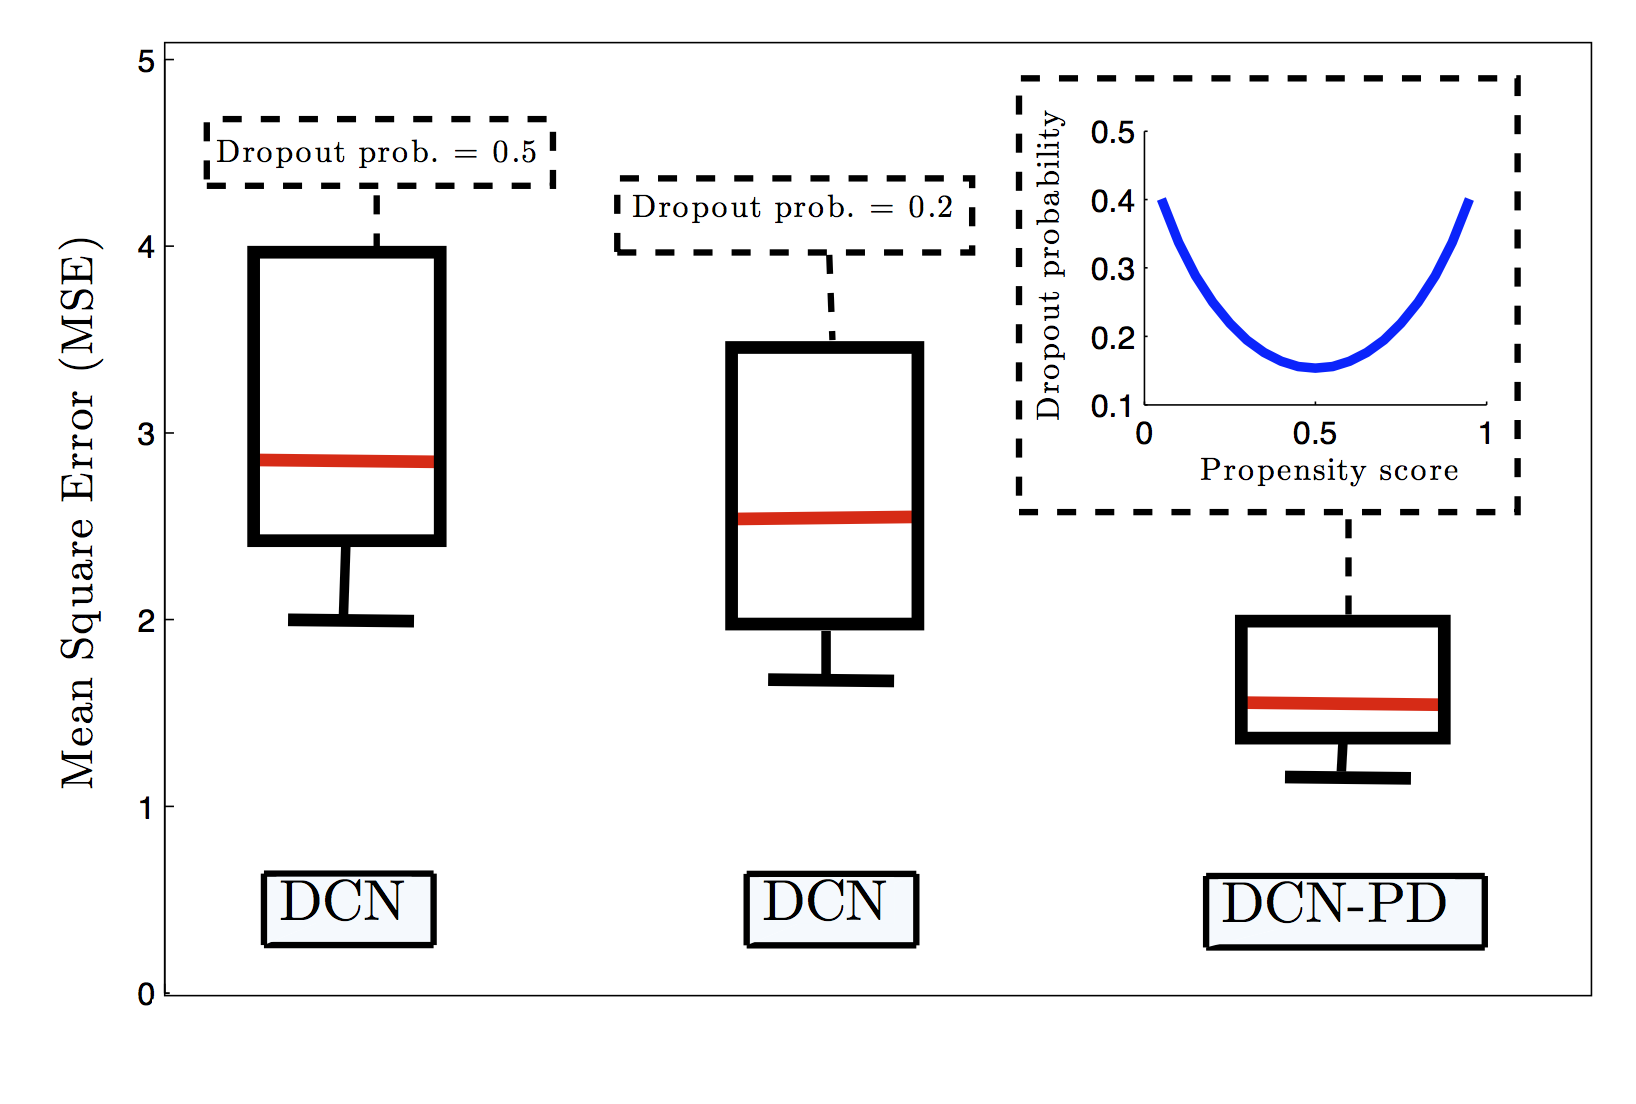
\includegraphics[width=0.8\textwidth]{figures/chapter-5/pd-boxplot.png}
	\caption{Comparison between the performance of a DCN with propensity-based dropout (right) and DCNs with regular dropout schemes (middle, left) in terms of the mean squared error (lower is better). The propensity-dropout has a regularising effect towards the selection bias and provides the model a higher degree of generalisation. }\label{fig:propensity-dropout-boxplot}
\end{figure}

As we can observe in the figure, our propensity-based dropout scheme provides a significant improvement over the alternative DCNs for which the  dropout probabilities are uniform throughout all samples in the training set. The result implies that the propensity-based dropout helps the DCN to generalise better to the true feature distribution when trained with an biased dataset such as IHDP (139 treated vs. 608 controlled subjects). Consequently, this suggest that propensity-dropout can be an effective regulariser for the task of counterfactual inference. 

In the following, we will look at the performance of DCNs and DCN-PDs in comparison to baseline methods and existing competing approaches. Table \ref{tab:dcn-pd-results} shows the 


\begin{table}[]
	\centering
	\begin{tabular}{@{}cc@{}}
		\toprule
		\textbf{Algorithm} & \textbf{MSE}   \\ \midrule
		k-NN               &   $5.30 \pm 0.30$ \\
		Causal Forest      &   $3.86 \pm 0.20$              \\
		BART               &   $3.50 \pm 0.20$           \\ 
		BNN                &   $2.45 \pm 0.10$           \\
		NN-4                &  $2.88 \pm 0.10$           \\
		DCN                &   $2.58 \pm 0.06$           \\
		DCN-PD             &   $2.05 \pm 0.03$          \\\bottomrule
	\end{tabular}
	\caption{Performance of Deep Counterfactual Networks (DCN) and Deep Counterfactual Networks with Propensity-Dropout (DCN-DP) in comparision with baseline methods and existing competing approaches}\label{tab:dcn-pd-results}
\end{table}



 In order to assess the marginal
by the proposed multitask model when combined with the propensity-dropout scheme, we compare the perfor- mance of DCN-PD with other state-of-the-art models in Table 1. In particular, we compare the MSE (av- eraged over 100 experiments) achieved by the DCN- PD with those achieved by k nearest neighbor match- ing (k-NN), Causal Forests with double-sample trees (WagerAthey, 2015), Bayesian Additive Regression Trees (BART) (Chipman et al., 2010; Hill, 2012), and Bal- ancing neural networks (BNN) (Johansson et al., 2016). (For BNNs, we use 4 layers with 200 hidden units per layer to ensure a fair comparison.) We also provide a direct com- parison with a standard single-output feed-forward neural network (with 4-layers and 200 hidden units per layer) that treats the treatment assignment as an input feature (NN-4), and a DCN with a standard dropout with a probability of 0.2. As we can see in Table 1, DCN-PD outperforms all the other models, with the BNN model being the most compet- itive. (BNN is a strong benchmark as it handles the selec- tion by learning a “balanced representation” for the input features (Johansson et al., 2016).) DCN-PDs significantly
performance gain achieved
Mean Square Error (MSE)
Dropout probability
%Deep Counterfactual Networks
 outperforms the NN-4 benchmark, which suggests that the multitask modeling framework is a more appropriate con- ception of causal inference compared to direct modeling by assuming that the treatment assignment is an input feature.



\section{Architecture Learning for DCN}
\subsection{Dataset}
\subsubsection{Synthetic}
\subsubsection{UNOS}

\subsection{Experiment Setup}

\subsection{Results}

\subsection{Conclusions}